\documentclass[tikz,border=4pt]{standalone}
\usepackage[T1]{fontenc}
\usepackage{lmodern}
\usetikzlibrary{arrows.meta,positioning,fit,backgrounds,calc}
\begin{document}
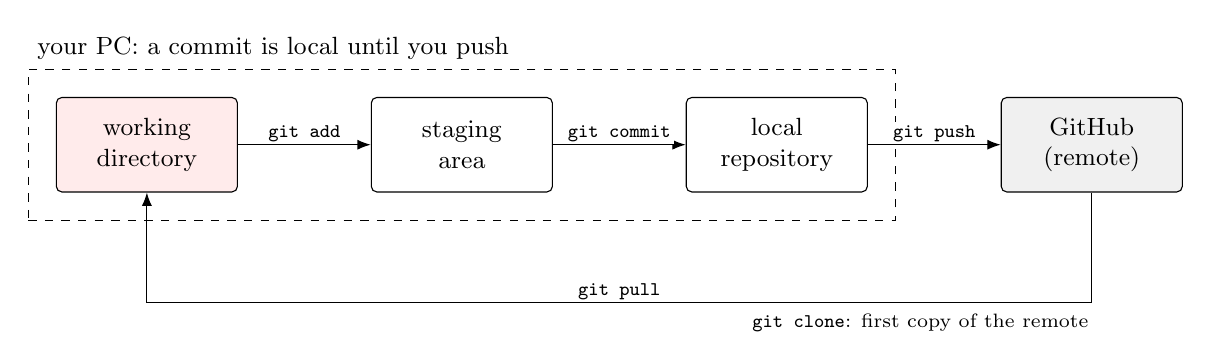
\begin{tikzpicture}[
  blk/.style={draw,rounded corners=2pt,minimum height=12mm,minimum width=23mm,align=center,font=\small,fill=white},
  ros/.style={blk,fill=red!8},
  ext/.style={blk,fill=gray!12},
  lab/.style={font=\scriptsize,fill=white,inner sep=1pt,align=center},
  >={Latex}]
\node[ros] (wd) at (0,0) {working\\directory};
\node[blk] (st) at (4,0) {staging\\area};
\node[blk] (lr) at (8,0) {local\\repository};
\node[ext] (gh) at (12,0) {GitHub\\(remote)};
\begin{scope}[on background layer]
\node[draw,dashed,inner sep=3.5mm,fit=(wd)(st)(lr)] (pc) {};
\end{scope}
\node[font=\small,anchor=south west] at (pc.north west) {your PC: a commit is local until you push};
\draw[->] (wd) -- node[lab,above]{\texttt{git add}} (st);
\draw[->] (st) -- node[lab,above]{\texttt{git commit}} (lr);
\draw[->] (lr) -- node[lab,above]{\texttt{git push}} (gh);
\draw[->] (gh.south) -- ++(0,-1.4) -| node[lab,pos=0.25,above]{\texttt{git pull}} (wd.south);
\node[lab,anchor=north east] at ($(gh.south)+(0.0,-1.5)$) {\texttt{git clone}: first copy of the remote};
\end{tikzpicture}
\end{document}
